\documentclass{beamer}

\usetheme{AnnArbor}
\usecolortheme{beaver}

\begin{document}

\title[OONI]{OONI: Open Observatory of Network Interference}
\author[Arturo Filast\`{o}]{{\bf Arturo Filast\`{o}}\inst{1} \and
	{Aaron Gibson}\inst{1} \and \\
	{Iain R. Learmonth}\inst{2} \and
	{Vasilis Ververi}\inst{2}}
\institute[Tor Project]{\inst{1} The Tor Project \and
           \inst{2} Open Rights Group}
\date{Day 3 / Lightning Talks} 

\begin{frame}
\maketitle
\end{frame}

\begin{frame}
	\frametitle{What is OONI?}
	\begin{itemize}
		\item{It’s a set of principles and test specifications for
			conducting network measurements.}
		\item{Measuring network irregularities that can be a symptom of
			internet censorship and surveillance since 2012.}
		\item{Uses a peer reviewed methodology, implemented using free
			software and publishing the data.}
	\end{itemize}
\end{frame}

\begin{frame}
	\frametitle{Interference in the Network\footnote{\tiny Image credit: \url{http://commons.wikimedia.org/wiki/File:Man_in_the_middle_attack.svg}}}
	\begin{center}
		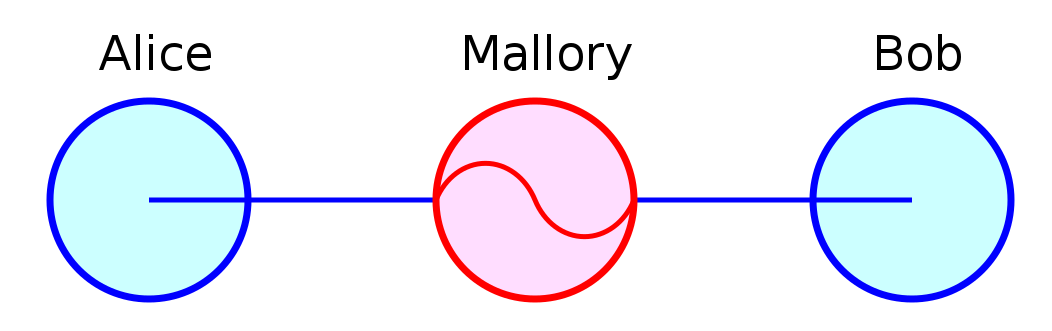
\includegraphics[width=0.7\textwidth]{mitm.png}
	\end{center}
	\begin{tabular}{ p{0.5\textwidth} p{0.5\textwidth} }
	\begin{itemize}
		\item{Traffic Manipulation}
			\begin{itemize}
				\item{Is my traffic being intercepted?}
				\item{DPI, Downgrade attacks, ...}
			\end{itemize}
		\end{itemize} &
		\begin{itemize}
			\item{Content Blocking}
			\begin{itemize}
				\item{What is being blocked?}
				\item{Unavailable websites, trigger keywords, ...}
			\end{itemize}
		\end{itemize}
\end{tabular}
\end{frame}

\begin{frame}
	\frametitle{Why is this important?}
	\begin{itemize}
		\item{OONI makes data available for everyone under an open
			license}
			\begin{itemize}
				\item{useful to journalists, researchers and activitists}
				\item{promotes transparency for network interference on the Internet}
			\end{itemize}
	\end{itemize}
\end{frame}

\begin{frame}
	\frametitle{Open Methodologies}
	\begin{itemize}
		\item{By having openly known and peer reviewed methodologies:}
		\begin{itemize}
			\item{the results produced have scientific value}
			\item{the research is reproducable and verifiable}
		\end{itemize}
		\item{Methodologies are described in plain English as well as in code}
	\end{itemize}
\end{frame}

\begin{frame}
	\frametitle{Test Focussed}
	\begin{itemize}
		\item{Plain English descriptions are written before code}
		\item{Allows for focus on the tests as opposed to a focus on implementation}
		\item{Allows for the construction of a taxonomy of surveillance, censorship and other interference}
	\end{itemize}
\end{frame}

\begin{frame}
	\frametitle{Open Implementation}
	\begin{itemize}
		\item{OONI's implementations are available as FLOSS}
		\item{Those interested in expanding it will be able to do so freely}
		\item{Allows it to be sustained as a base for future work}
		\item{A FLOSS tool has the most likely chance of being studied and improved by the research community}
	\end{itemize}
\end{frame}

\begin{frame}
	\frametitle{Low barrier to entry}
	\begin{itemize}
		\item{Probes are hosted by volunteers}
		\item{Anyone can volunteer to host a probe}
		\item{Volunteers can choose which tests they run}
		\item{Volunteers can choose how much data they want to submit}
	\end{itemize}
\end{frame}

\begin{frame}
	\frametitle{Open Data}
	\begin{itemize}
		\item{The rate of discovery and scientific progress is accelerated by better access to data}
		\item{All of the data collected by OONI is released to the public under an open license}
		\item{This allows anybody to freely use and republish this information as they wish without restriction}
		\item{High-level summaries are not enough}
	\end{itemize}
\end{frame}

\begin{frame}
	\frametitle{Users}
	\begin{itemize}
		\item{OONI has been used by a series of independent researchers in order to conduct their measurements}
			\begin{itemize}
				\item{Analysis of Iran Wikipedia censorship (May 2013)}
				\item{WCMT: Web Censorship Monitoring Tool (June 2013)}
				\item{ Measurement of internet censorship in Indonesia (October 2013)}
			\end{itemize}
	\end{itemize}
\end{frame}

\begin{frame}
	\frametitle{Get Involved!}
	Join the fight against surveillance and censorship by adopting
	an ooniprobe. Feed it power and internet packets to watch it grow!

	\ 

	{\Large\bf ``Adopt an ooniprobe": 1800 Tomorrow at the Noisy Square Assembly}

	\ 

	\url{http://ooni.torproject.org/}
\end{frame}	

\end{document}
